\documentclass[11pt, 
%oneside, % Two side (alternating margins) for binding by default, uncomment to switch to one side
ngerman,
%singlespacing, % Single line spacing, alternatives: 
%onehalfspacing,
%or 
doublespacing,
%draft, % Uncomment to enable draft mode (no pictures, no links, overfull hboxes indicated)
%nolistspacing, % If the document is onehalfspacing or doublespacing, uncomment this to set spacing in lists to single
%liststotoc, % Uncomment to add the list of figures/tables/etc to the table of contents
%toctotoc, % Uncomment to add the main table of contents to the table of contents
%parskip, % Uncomment to add space between paragraphs
%nohyperref, % Uncomment to not load the hyperref package
%headsepline, % Uncomment to get a line under the header
chapterinoneline, % Uncomment to place the chapter title next to the number on one line
consistentlayout, % Uncomment to change the layout of the declaration, abstract and acknowledgements pages to match the default layout
]{scrartcl}
\usepackage{ngerman}
\usepackage{graphicx}
\usepackage{hyperref} 
\usepackage[figure]{hypcap}
\usepackage{url}
\begin{document}
\author{Niels Gundermann}
\title{Kommunikation zwischen entkoppelten Java-Modulen über strukturell typkonforme Objekte

%Verwendung strukturell typkonformer Java-Objekte in voneinander entkoppelten Modulen 
}
\maketitle
\section{Einleitung}
Die Modularisierung ist ein gängiges Mittel zur Beherrschung komplexer Softwaresys\-teme. Die Kommunikation zweier Module wird dabei durch eine vorab definierte Schnitt\-stelle gewährleistet. Bei der Kommunikation kann es sich lediglich um den Aufruf eines Dienstes handeln, oder um einen Datenaus\-tausch über so genannte Transfer-Objekte.\\\\
In der Programmiersprache Java wer\-den diese Schnittstellen im Allgemeinen häufig als Interfaces definiert und gliedern sich somit in die Typ-Hierarchie des Programms ein. Soll ein Modul \emph{A} mit einem Modul \emph{B}  kommunizieren, so müssen beide Module ein Interface \emph{I} als Schnittstelle kennen und sind damit abhängig von diesem. Wenn es zu einem Datenaustausch über \emph{I} kommen soll, so müssen die beiden Module darüber hinaus die Typen kennen, durch die die Transfer-Objekte abgebildet werden (Transfer-Typen).\\\\
Die Konformität der Typen (Transfer-Typen und Interfaces) wird in Java auf nominaler Ebene, also auf der Basis der Bezeichnung des jeweiligen Typs, sichergestellt (Nominale Typkonformität).
Die dadurch entstehende Abhängigkeit führt zu einer Behinderung möglicher paralleler Arbeiten an diesen Modulen - insbesondere dann, wenn die Schnitt\-stelle im Zuge der Arbeiten angepasst werden muss und die beiden Module im Verantwor\-tungs\-bereich unterschiedlicher Entwicklerteams liegen.\\\\ 
Ein anderer Ansatz zur Sicherstellung der Typkonformität beruht auf dem Abgleich der strukturellen Eigenschaften von Typen (Strukturelle Typkonformität). Dabei werden die Transfer-Typen und Interfaces, die für die Kommunikation zwischen zwei Modulen (\emph{A} und \emph{B}) benötigt werden, innerhalb beider Module definiert, sodass jedes Modul seine eigenen Typen bereitstellt. Die beiden Module wären somit voneinander und von einer gemeinsamen Schnitt\-stelle (\emph{I}) syntaktisch unabhängig.
%, da die Konformität zwischen den Typen, nicht anhand der Bezeichnung gewährleistet wird, sondern auf der Basis  gleicher Strukturen der in beiden Modulen definierten Interfaces und Transfer-Typen für die jeweilige Kommunikation.
\\\\
Es gab bereits Überlegungen dazu, wie eine strukturelle Typkonformität in der Program\-mier\-sprache Java umgesetzt werden könnte (vgl. \cite{whiteoak}, \cite{structconfjava}). Die Arbeit von Läufer et al. (\cite{structconfjava}) beschränkt sich dabei jedoch nur auf die Konformität zwischen Klassen und Interfaces und bedingt eine Anpasssung des Java-Compilers. Bei der Lösung von Gil et al. (\cite{whiteoak}) handelt es sich um eine Spracherweiterung, was die Integration in bestehende Systeme erheblich erschwert.
% Die dafür notwendigen Erweiterung beschränkten sich jedoch nur auf die Konformität zwischen Klassen und Interfaces (vgl. \cite{structconfjava}) oder erfordern eine Spracherweiterung (vgl. \cite{whiteoak}).
\\\\ 
Die vorliegende Arbeit befasst sich mit einem Ansatz der einerseits als Java-Bibliothek integriert werden kann und andererseits auch die Konformität zwischen Klassen als Transfer-Typen herstellen soll. 
Aufgrund der Tatsache, dass die Methoden strukturell typkonformer Objekte, in unterschiedlichen Modulen auch unterschiedlich implementiert werden können, muss entschieden werden, welche der Implementierung letztendlich ver\-wendet werden soll. Auf dieses Problem wird ein besonderer Fokus innerhalb dieser Arbeit gelegt.
Dies betrifft natürlich nicht nur Methoden-Implementierungen in Klassen, sondern auch default-Methoden in Interfaces.

\subsection{Problembeschreibung}\label{problembeschreibung}
In dieser Arbeit werden zwei Szenaien betrachtet, die unterschiedliche Probleme aufzeigen. In beiden Fällen wird ein Ausschnitt aus einem System beschrieben, dessen Aufbau den Prinzipien einer strengen Schichtenarchitektur folgt  (siehe \ref{architektur}).
\subsubsection{Szenario 1}
Auf architektonischer Ebene kann das erste Szenario, wie im Abbildung \ref{fig:problem} folgt dargestellt werden.
\begin{figure}[h]
  \centering
  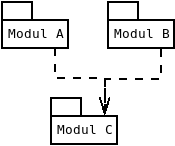
\includegraphics[scale = 0.7]{pics/problemS1Abstrakt.png}
  \caption{Problem: Szenario 1}
  \label{fig:problem}
\end{figure}
Die Module \emph{A} und \emph{B} liegen architektonisch auf der gleichen Ebene und dürfen somit keine direkte Abhängigkeiten aufweisen. Das Modul \emph{C} stellt eine Abstraktionsebene dar, die für das gesamte System verwendet wird. Änderungen an diesem Modul würden demnach nicht nur die Module \emph{A} und \emph{B} betreffen, sondern auch noch weitere Module, die in Abbildung \ref{fig:problem} nicht aufgeführt sind. Zudem soll zusätzlich davon ausgegangen werden, dass die Module \emph{A} und \emph{B} im Verantwortungsbereich eines Eintwicklerteams \emph{E1} liegen, während das Modul \emph{C} im Verantwortungsbereich eines Entwicklerteams \emph{E2} liegt.\\\\
Nun wird eine abstrakte Klasse aus Modul \emph{C} in Modul \emph{B} konkret implementiert. Weiterhin werden Objekte, die in Modul \emph{B} erzeugt werden in Modul \emph{A} verwendet. Die Verwendung erfolgt jedoch über die abstrakte Klassendefinition aus Modul \emph{C}.\\\\
Aufgrund einer geänderten Anforderung muss innerhalb von Modul \emph{A} eine Information genutzt werden, die bereits in der konkreten Implementierung aus Modul \emph{B} vorliegt, aber nicht in der abstrakten Implementierung aus Modul \emph{C} zur Verfügung steht. In diesem Szenario gäbe es aufgrund der nominalen Typkonformität folgenden Lösungsvarianten:
\begin{enumerate}
\item Die abstrakte Impementierung wird um diese Information erweitert.
\item Es wird eine weitere Abstraktionsschicht zwischen den beiden vorliegenden Schichten eingebaut.
\end{enumerate}
Beide Lösungsvarianten führen zu relativ hohem Anpassungsaufwand, wenn man bedenkt, dass die benötigte Information bereits zur Verfügung steht.
\subsubsection{Szenario 2}
Das zweite Szenario bezieht sich auf eine Serviceorientierte Architektur (siehe \ref{sarchitektur}).
Abbildung \ref{fig:problem2} zeigt den angenommenen Ausschnitt aus einem System. 
\begin{figure}[h]
  \centering
  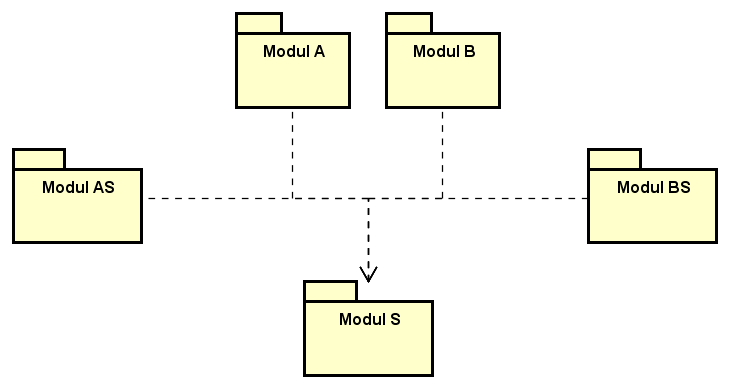
\includegraphics[scale=0.7]{pics/problemS2Abstrakt.png}
  \caption{Problem: Szenario 2}
  \label{fig:problem2}
\end{figure}\\
Hierbei wird von einem Broadcast Serviceaufruf ausgegangen. Sas bedeutet, dass es eine Service-Schittstelle gibt, die in mehreren Modulen implementiert wird. Die Aufrufer liegen in diesem Fall in Modul \emph{A} und \emph{B}, während die Service-Schnittstelle in Modul \emph{S} liegt. Die weiteren Module beinhalten unterschiedliche Implementierungen des augerufenen Services. Weiterhin ist anzunehmen, dass alle Module im Verantwortungsbereich unterschiedlicher Entwicklerteams liegen.\\\\
Nun ist davon auszugehen, dass innerhalb von Modul \emph{A} eine weitere Information durch den Service bereitgestelt werden soll. Hierbei gibt es folgende Lösungsansätze:
\begin{enumerate}
\item Die Service-Schnittstelle wird erweitert.
\item Es wird eine neue Service-Schnittstelle geschaffen, die künfitg nur von Modul \emph{A} verwendet wird.
\end{enumerate}
Beide Lösungsansätze erfordern wiederrum erheblichen Aufwand und Koordination zwischen den Entwicklerteams. Daber ist zu erwähnen, dass der zweiter Lösungsansätz etwas weniger Aufwand erfordert, da die Entwicklerteams, deren Service-Implementierungen ohnehin in Modul \emph{A} keine Verwendung finden, nicht beteiligt sind. 

\section{Typen und Typkonformität}
\cite{types}
\subsection{Typen in Java}
\subsection{Typkonformität in Java}
\cite{structconfjava}, \cite{compoundtypes}
\subsection{Formale Definition struktureller Typkonformität in Java}
\cite{structconfjava}
\section{Softwarearchitektur}
\cite{Bas13}
\subsection{Schichtenarchitektur}\label{architektur}
\cite{modanwendungen}
\subsection{Serviceorientierte Architektur}\label{sarchitektur}
\cite{modanwendungen}
\subsection{Schnittstellen}
\cite{Bas13}, \cite{Bus96}
\section{Lösungsansätze}
\subsection{Bestehende Lösungen}
In den folgenden Kapiteln wird auf die Lösungsmöglichkeiten der in \ref{problembeschreibung} beschriebenen Szenarien mit den bestehenden Lösungen nach \cite{structconfjava} und \cite{whiteoak} eingegangen. Die hier beschriebenen Lösungsansätze basieren lediglich auf den theoretischen Ausführungen bzgl. der allgemeinen Ansätze. Es wurde kein praktischer Nachweis in Form einer Implementierung erbracht, der die theoretischen Grundlagen aus \cite{structconfjava} und \cite{whiteoak} bestätigt. Das Ziel dieses Abschnittes der Arbeit ist es, grundlegende Konzepte, die in den nachfolgenden Lösungsansätzen enthalten sind, aufzunehmen und weiterzuentwickeln.
\subsubsection{Erweitung des Java-Compilers}
\cite{structconfjava}

\subsubsection{WHITEOAK}
\cite{whiteoak}
\subsubsection{REST/SOAP}
\subsection{Interfaces als Schnittstellen-Typ}
\subsubsection{Umsetzung mit dynamischen Proxies}
\cite{proxy}
\subsection{Klassen als Schnittstellen-Typ}
\subsubsection{Umsetzung mit cglib}
\cite{cglib}
\section{Diskussion}
\subsection{Vergleich mit bestehenden Lösungen}
\subsection{Verwendung definierter Methoden in Transfer-Objekten}
\section{Fazit}

\bibliography{bib}{}
\bibliographystyle{plain}
\nocite{*}
\end{document}